Sensible DTU was an experiment conducted as part of the ongoing interdisciplinary research project \textit{Social Fabric} at Copenhagen University (UCPH) and DTU Compute of The Technical University of Denmark (DTU), which ran from September 2013 to January 2015 (2.5 years). In the experiment, 863 undergraduate students at DTU gave informed consent to participate. Participants were predominantly male (78.8\%), of average age 21.7 (SD 2.8) years, distributed across all study lines, and were primarily 1st year students (59.2\%) and 2nd year students (30.2\%). Remaining students were either 3rd year students or students for which a year was not reported. Participants were provided a NEXUS smartphone for personal use, which was reprogrammed to continuously collect social behavioral data through multiple channels\mcite{sensibleDTUdocumentation, stopczynski2014a}. Tab. \ref{tab:datatypes} gives an overview of which social behavioral data were collected.

\begin{table}[b!]
	\centering
	\bgroup
	\def\arraystretch{1.2}
	\begin{tabular}{R{4.0cm}|C{2.5cm}C{3cm}}
		\toprule
		\textit{Datatype} & \textit{Sample period} & \textit{Used in this study}\\
		\hline\hline
		GPS-location         &  15 minutes &  \textbf{Yes} \\
		WiFi-scans           &  10 minutes &  No \\
		Bluetooth-scans      &  5 minutes  &  \textbf{Yes} \\
		Phone calls          &  -          &  \textbf{Yes} \\
		Text messages        &  -          &  \textbf{Yes} \\
		Facebook data        &  -          &  No \\
		Screen on/off events &  -          &  \textbf{Yes} \\
		\bottomrule
	\end{tabular}
	\egroup
	\caption{\label{tab:datatypes}Overview of the datatypes which were collected through the administered smartphones, and which are used in this study. Niether channel provides written or spoken content. The Facebook channel includes friends, groups, interests, likes, political orientation, religion and more.}
\end{table}

The experiment saw its largest volume of activity in the spring of 2014, where 526 students were actively using the provided smartphone as their primary device (active on more than 75\% of days through the period, see Fig. \ref{fig:data_activity}).

\begin{figure}[h!]
	\centering
	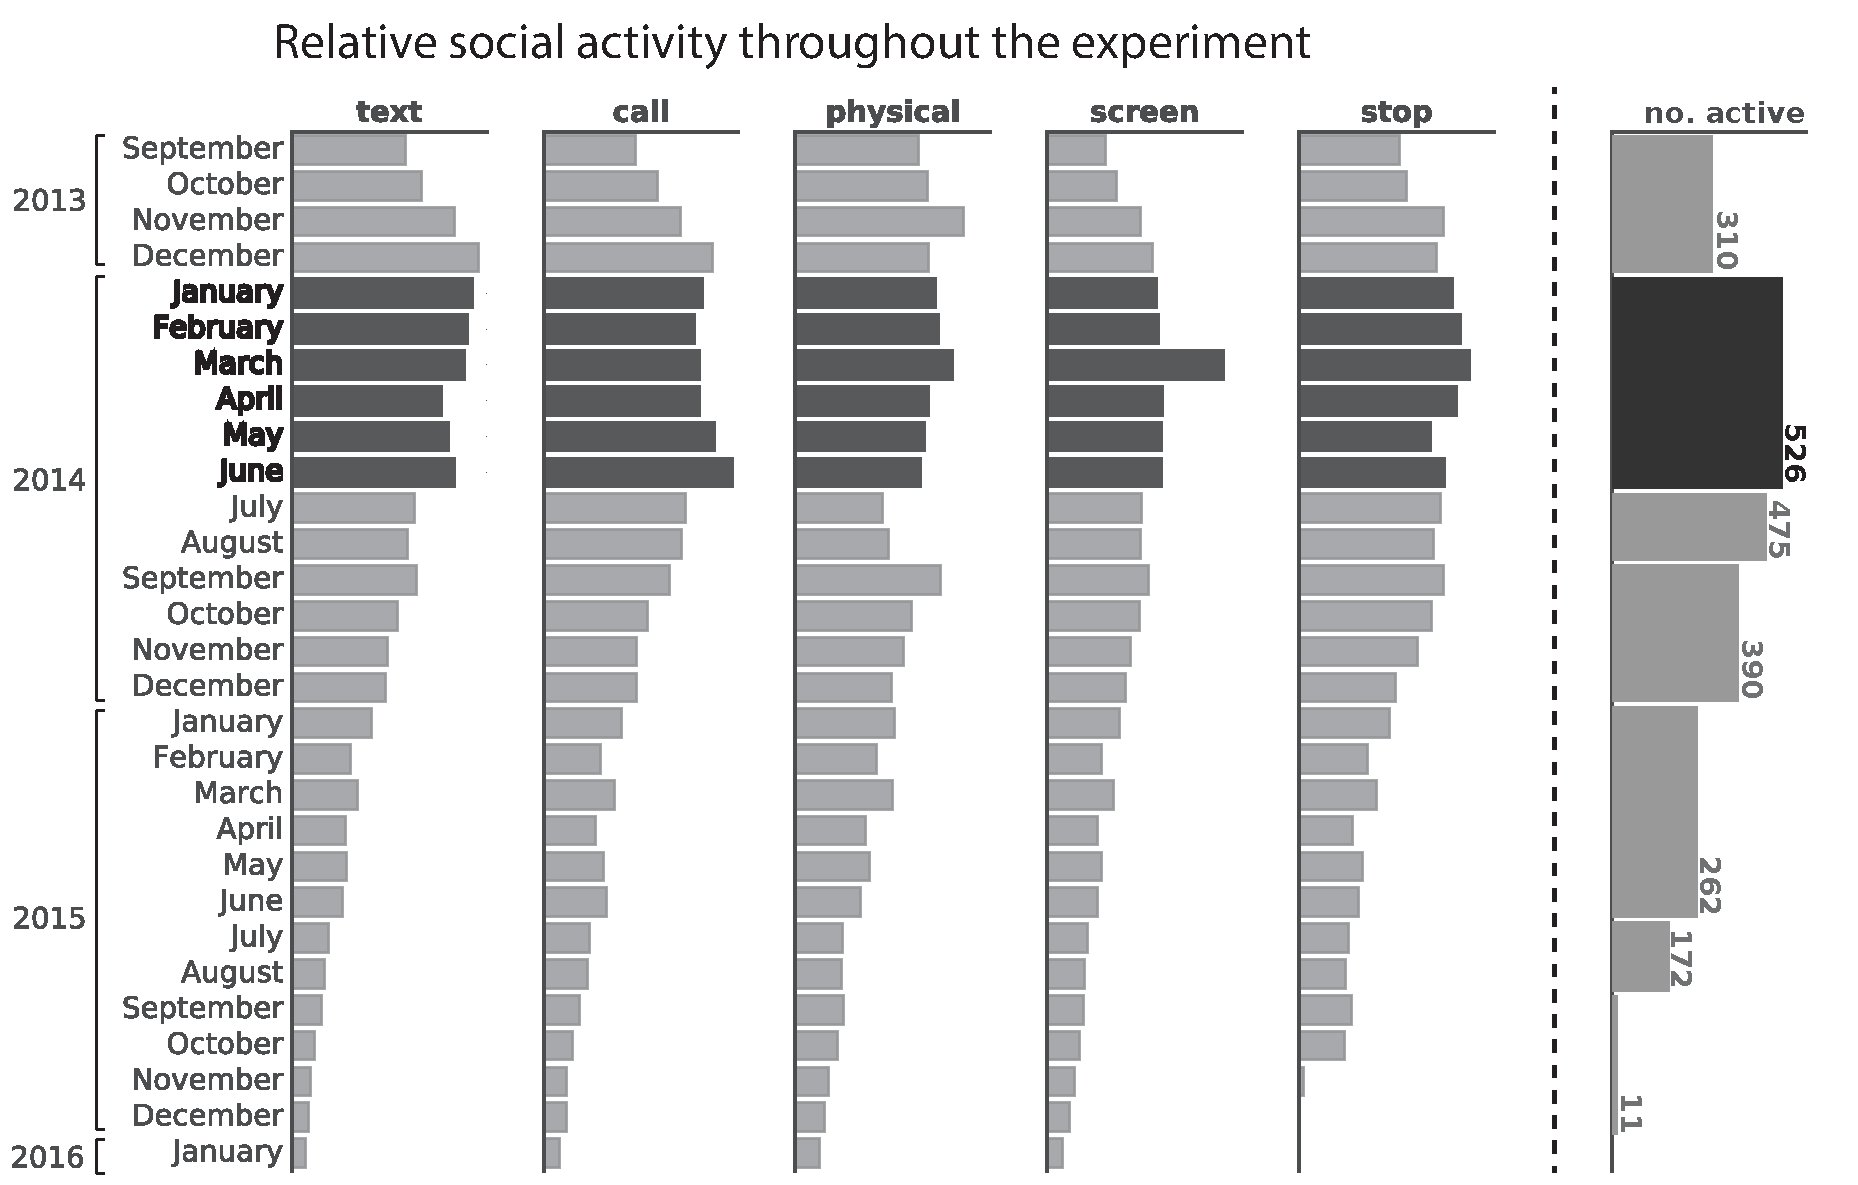
\includegraphics[width=0.8\linewidth]{figures/data_activity}
	\caption{\label{fig:data_activity}An overview of the amount of activity tracked in the respective months of the experiment. The months marked in bold represent those with which the data used in this study is associated. The far right bar plot show the number of students in each semester and summer holiday, which are active on more than 75\% of days through the period.}
\end{figure}

As described in Sec. \ref{subsubsec:behaviorAndPersonality}, behavioral inconsistency sets a limit for the level of mutual information, or correlation, there may be found between a personality trait obtained through a questionnaire, and a specific type of behavior. To mitigate such influence, data originating only from school weeks in the spring semester of 2014 is selected for analysis, based on the assumption that this provides the highest degree of self-similarity in the data. Similar subsets, e.g. from exam periods or holiday weeks, could also have been chosen, but would contain less data since these are narrower spans of time.

Before receiving the phone, participants were required to fill out a baseline questionnaire. It included the Big Five (BF) questionnaire which was used in this study to obtain BF profiles for each subject (see Sec. \ref{subsubsec:dimensionsOfPersonality}). The BF questionnaire was filled out for each participant no later than december 20th of 2013\mcite{sensibleDTUdocumentation}. The notion raised in Section \ref{subsubsec:behaviorAndPersonality} that behavior and personality are not constants provides a compelling argument that they should be measured as close in time as possible, which gives another reason for choosing to use only behavioral data from the spring semester of 2014.
%Fig. \ref{fig:big_five_violin_plots} shows violin plots for the different Big Five traits in the dataset.

% \begin{figure}
% 	\centering
% 	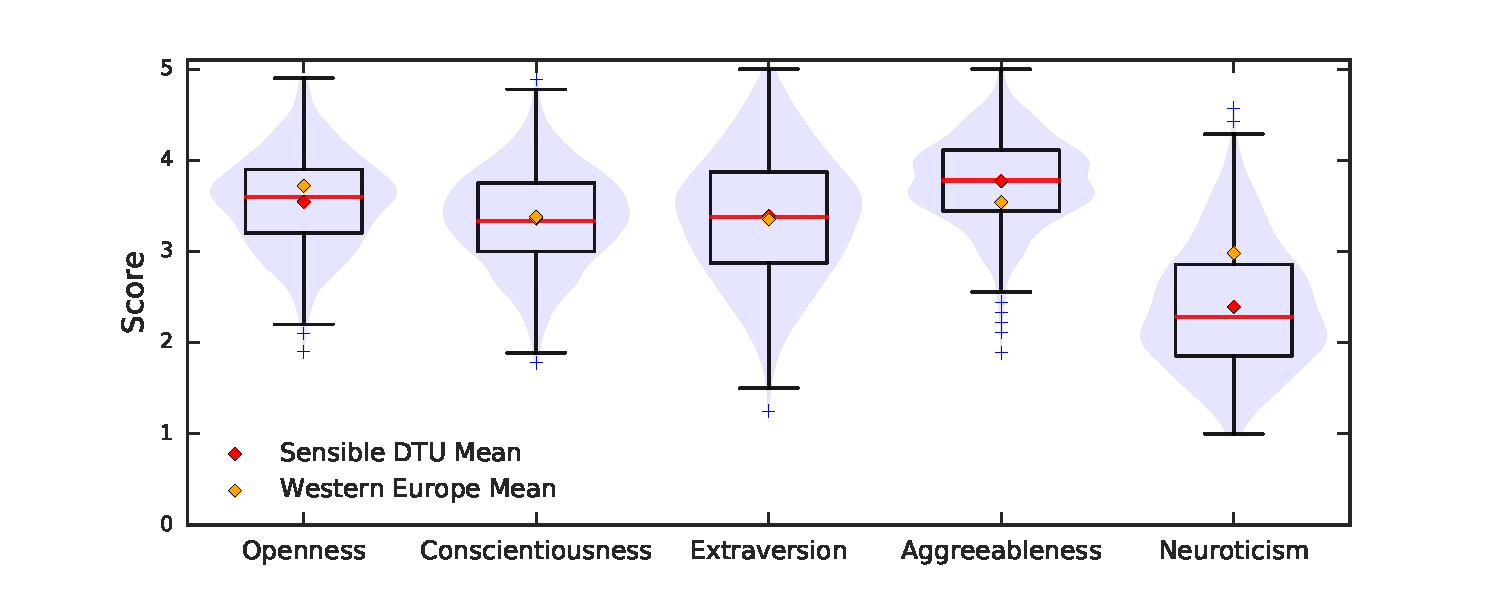
\includegraphics[width=0.8\linewidth]{figures/big_five_violin_plots}
% 	\caption{\label{fig:big_five_violin_plots}Violin plots of Big Five personality traits in the Sensible DTU data. Summary statistics of the format \texttt{mean} (\texttt{SD}) are: openness 3.58 (0.52); conscientiousness 3.44 (0.51); extraversion 3.15 (0.53); agreeablenes 3.64 (0.51); neuroticism 2.59 (0.65). Red dots represent mean values in this study and orange diamonds are mean in Western Europe (mixed population)\cite{schmitt2007geographic}.}
% \end{figure}

Researchers in the Social Fabric project also has access to administrative data such birth year, courses, drop-out and most notably grades, none of which, however, were used in this study.

\subparagraph*{Privacy and data access} Given the sensitive information contained, or easily extracted, from this data despite all reference to personal identity having been removed, strict access rules to the data are imposed. Researchers are obliged to sign a non-disclosure aggreement (NDA) and raw data is not to be contained on private of public machines outside of the EU. Data is accessed in JSON format through the Data Viewer API at \texttt{sensible.dtu.dk/apps/data\_viewer} with a valid research token, or through a virtual IPython Notebook environment hosted at \texttt{raw.sensible.dtu.dk}, where data is served as Numpy MaskedArray type for efficiency which easily converts to Pandas DataFrame type, Numpy 2D array or similar matrix-like types (see Sec. \ref{subsec:behavioralDataPreprocessing} for technical reference). Researchers working outside of the EU are restricted to work with the data remotely through the virtual IPython Notebook environment, which is, conveniently, also the faster alternative.